\documentclass[10pt]{article}
\usepackage[T1]{fontenc}
%\usepackage[utf8]{inputenc}
\usepackage[french]{babel}
\usepackage{graphics}
\title{Page de garde du TER et du M\'emoire de l'Universit\'e des Antilles-Guyane}
\newcommand{\LOL}[1]{\mbox{\raisebox{1em}{\rotatebox{-90}{:-)}}\raisebox{2em}{\rotatebox{-90}{:-)}}\hspace{-2ex}\rotatebox{-90}{:-)}}~#1~%
\mbox{\raisebox{2em}{\rotatebox{-90}{:-)}}\hspace{-2ex}\rotatebox{-90}{:-)}\raisebox{1em}{\rotatebox{-90}{:-)}}}}

\usepackage[pdftex,colorlinks]{hyperref}
\hypersetup{%
   pdfauthor=C\'edrick \textsc{Copol},%
   pdftitle=Page de garde du TER et du M\'emoire de l'Universit\'e des Antilles-Guyane%
}

\author{C\'edrick \textsc{Copol}}

\begin{document}
\maketitle
\tableofcontents

\section{Contenu }
Pour faire la page de garde vous trouverez les fichiers suivants :

\begin{itemize}
 \item 	apercu.tex
 \item	PagedegardeUAG-doc.pdf \og la documentation que vous lisez en ce moment \fg{}
 \item	nouveau\_logo\_uag.eps
 \item	pagedegardeUAG.sty
 \item	apercuTer.pdf \og r\'esultat que vous devez obtenir pour un TER \fg
 \item	apercuMemoire.pdf \og r\'esultat que vous devez obtenir pour un M\'emoire \fg
\end{itemize}

\section{Mode d'emploi }

\begin{enumerate}
 \item  Placez dans votre dossier de travail, celui contenant votre .tex, les fichiers
	nouveau\_logo\_uag.eps
	pagedegardeUAG.sty


 \item  Editez votre .tex

  \item Pr\'eciser au besoin a4paper , dans \textbackslash documentclass[a4paper]\{\ldots\}

 \item  Pour charger l'extention \emph{pagedegardeUAG} taper dans le pr\'eambule
\mbox{\textbackslash usepackage[X]\{pagedegardeUAG\}}
	o\`u X prend l'une de ces 2 valeurs en fonction de ce que vous pr\'eparer \LOL{bien-sur}:
		\begin{itemize}
		    \item ter
		    \item memoire
		\end{itemize}.

Quoi de plus parlant qu'un exemple ? \LOL{RIEN}

	    Vous pr\'eparez un \og ter \fg{} alors mettez 
	\mbox{\textbackslash usepackage[ter]\{pagedegardeUAG\}}.

	    Vous pr\'eparez un \og memoire \fg{} alors mettez 
	\mbox{\textbackslash usepackage[memoire]\{pagedegardeUAG\}}.

	Les classes support\'ees pour l'instant sont :
	\begin{itemize}
		\item article
		\item report
		\item book
	\end{itemize}
		(pour les autres il ne vous reste qu'\`a \LOL{essayer} )

 \item  Mettez dans le pr\'eambule 
	\begin{itemize}
		\item \mbox{\textbackslash usepackage\{xcolor\}}
		\item \mbox{\textbackslash usepackage\{graphicx\}}
		\item \mbox{\textbackslash usepackage\{pstricks,pst-grad\}}
	\end{itemize}
 \item  Et enfin renseignez les commandes suivantes :
	\begin{itemize}
	\item \mbox{\textbackslash email\{votreadress@trucmuche.chose\}}
		\item \mbox{\textbackslash author\{Pr\'enom NOM\}}
		\item \mbox{\textbackslash annee\{2008-2009\}}
		\item \mbox{\textbackslash Encadrant\{Mme, Mlle, M. Prof encadrant\}}
		\item \mbox{\textbackslash title\{ \}}
	\end{itemize}

 \item  Mettre la commande \mbox{\textbackslash maketitle} apr\`es \mbox{\textbackslash begin\{document\}}.

 \item  Attention pour obtenir le r\'esultat attendu vous devez compiler avec \LaTeX{} puis dvips puis ps2pdf (ou pstopdf).
       \LOL{Comment faire ?} Cherchez dans votre \'editeur de texte pr\'ef\'er\'e d\'edi\'e \`a \LaTeX, il s'aura le faire. 

 \item  Bonne journ\'ee en esp\'erant que sa fonctionne.
   Je vous remercie d'utiliser mon extension et bien-sur :
			BONNE CHANCE !!
\end{enumerate}

\section{R\'esolution de probl\`eme}
\subsection{Windows mon cher windows}

	Cette section ne concerne que les utilisateur de Windows (peut-\^etre Mac mais je n'avais personne pour tester). Alors les autres passez votre chemin.
	Il faut indiquer a MiK\TeX{} qu'il doit utiliser un format A4 mais un vrai format A4.
	Pour cela suivez le guide:

Cliquez sur le menu D\'emarrer puis sur \og tous les programmes\fg{}. Cherchez MiK\TeX{} 2.7(ou une autre version), un menu d\'eroulant s'ouvre avec ceci Browse Packages, 
Previewer, Settings et Update. Cliquez sur \og Settings \fg{} la fen\^etre \ref{image} s'ouvre :


\begin{figure}[h]
\hspace*{-2cm}  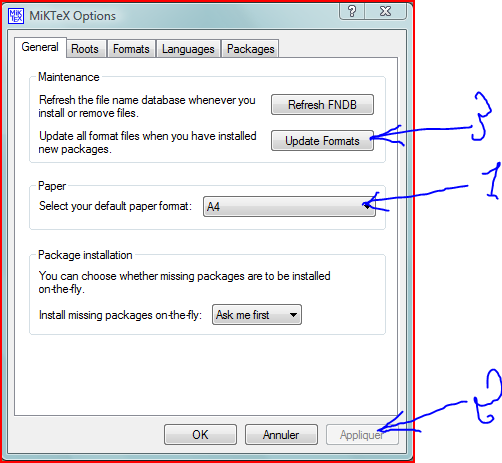
\includegraphics{miktex_option.png}
\caption{MiKTEX Settings}\label{image}
\end{figure}
\begin{description}
 \item[\'Etape 1] choisir A4 et non A4(size)
 \item[\'Etape 2] cliquez sur Appliquer
 \item[\'Etape 3] cliquez sur Update formats
 \end{description}



\subsection{Probl\`emes possibles}

Cette section est  relatif aux probl\`emes rencontr\'ees avec l'ancienne version (celle d'avril 2009) il est fort possible
 que ces probl\`emes aient disparus.\\
	Le cadre bleu n'est pas adjacent au bord droit de la feuille

\begin{itemize}
 \item  enlever l'option twoside dans \textbackslash documentclass.
 \item probl\`eme du aux extensions \emph{geometry}, \emph{fullpage} enlever les s'il ne sont pas utilis\'e.
 \item  Il peut \^etre n\'ecessaire d'\'ecrire\\ 
			\mbox{\textbackslash usepackage\{amsmath,amsfonts,amssymb,amsthm\}}
		 au lieu de \mbox{\textbackslash usepackage\{amsmath\}} \mbox{\textbackslash usepackage\{amsfonts\}} \mbox{\textbackslash usepackage\{amssymb\}} \mbox{\textbackslash usepackage\{amsthm\}}.
\end{itemize}

Si malgr\'e mes explications rien ne marche modifier directement le fichier apercu.tex .
Ainsi vous aurez un fichier ne contenant que la page de garde et un autre contenant votre travail, ou compiler chez un ami pour qui cela fonctionne.

\end{document}